\begin{frame}
\frametitle{The density of time nodes does not drive the group parameters}
\begin{columns}
    \column[t]{0.45\textwidth}
    \begin{block}{Group half-lives:}
        \begin{figure}[!ht]
            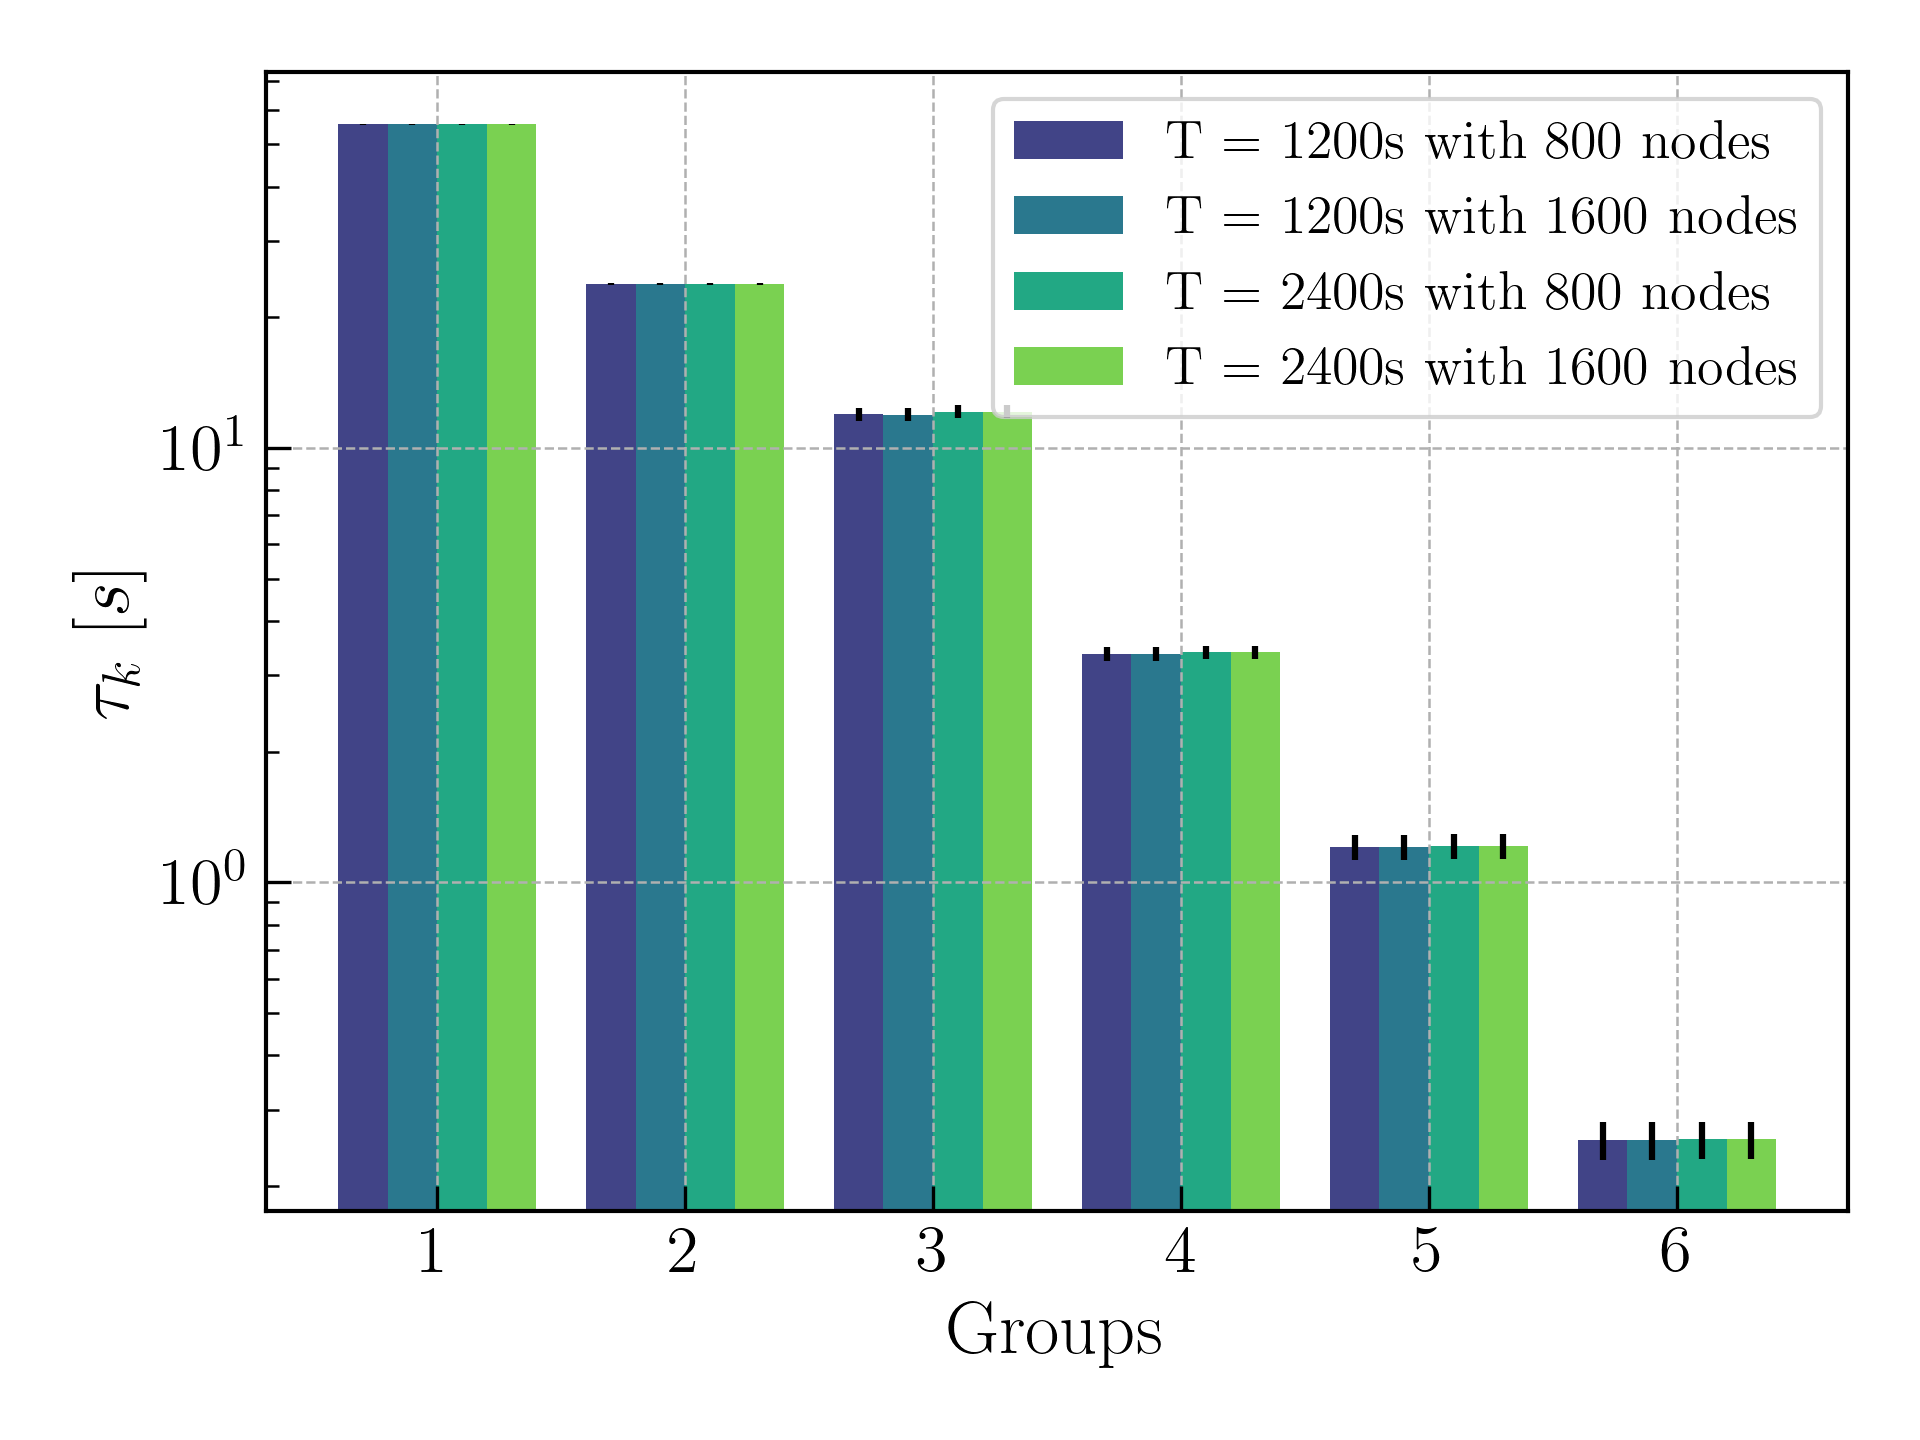
\includegraphics[width=1.0\linewidth]{../images/halflives_detailed_decay.png} 
            \caption{$\tau_k$ for each \gls{DNP} group $k$ after a thermal saturation irradiation of $^{235}$U using the 0D scaled model.}
        \end{figure} 
    \end{block}
    \column[t]{0.45\textwidth}
    \begin{block}{Group yields:}
        \begin{figure}[!ht]
            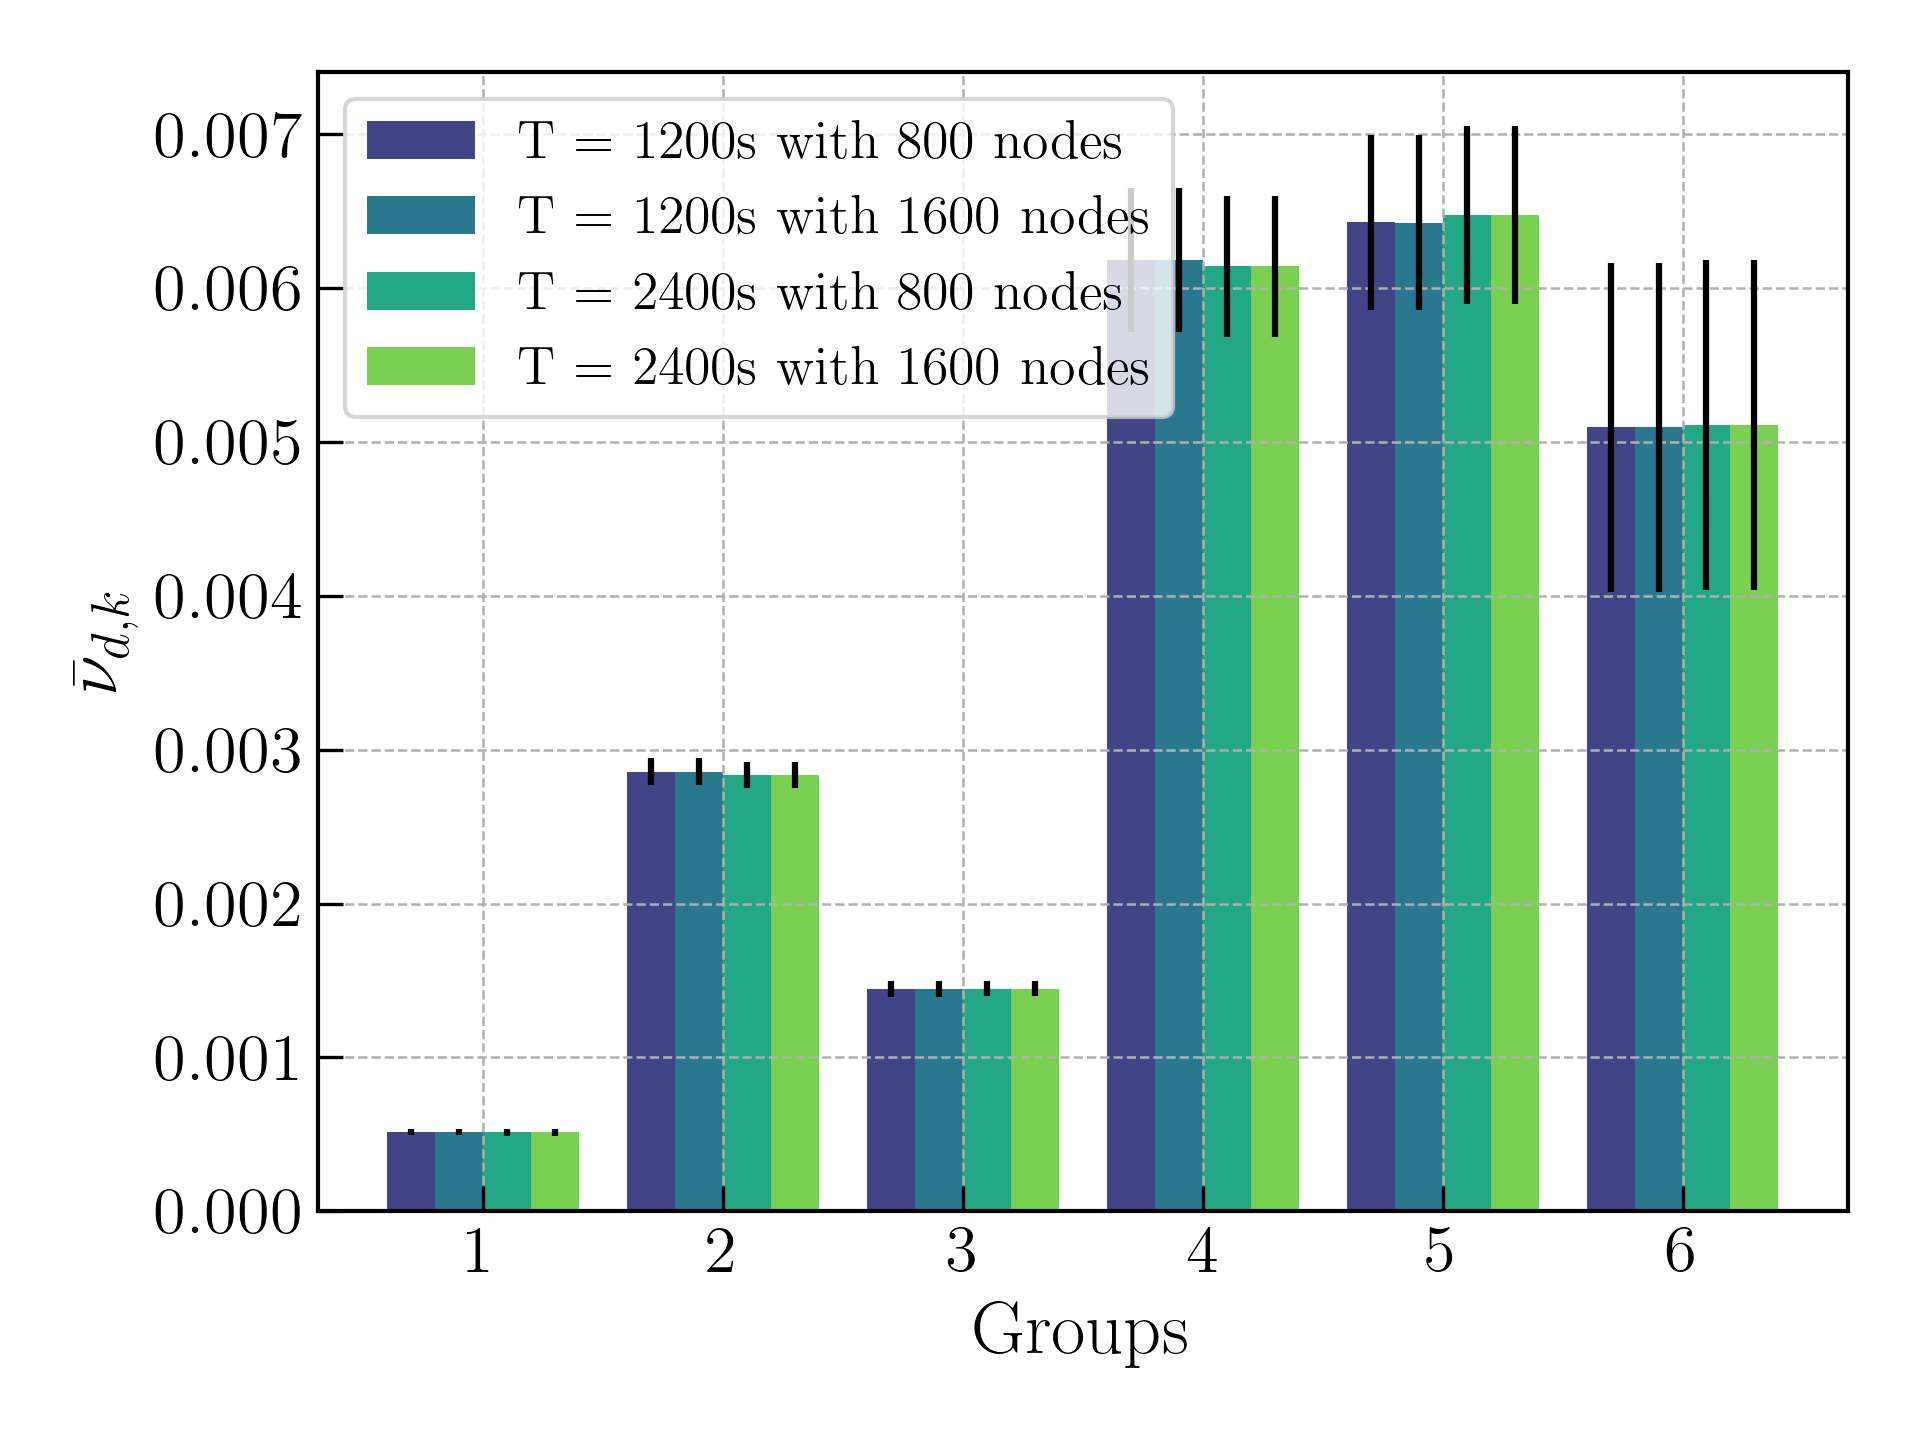
\includegraphics[width=1.0\linewidth]{../images/yields_detailed_decay.png} 
            \caption{$\bar{\nu}_{d,k}$ for each \gls{DNP} group $k$ after a thermal saturation irradiation of $^{235}$U using the 0D scaled model.}
        \end{figure} 
    \end{block}
\end{columns}
\textbf{The number of nodes has a small impact on the \gls{DNP} group parameters, whereas the total decay time causes larger differences.}
\end{frame}